Quoting @mwl@io.mwl.io: \url{https://io.mwl.io/@mwl/109881793335623363}
\#retoot

\begin{figure}
\centering
\pandocbounded{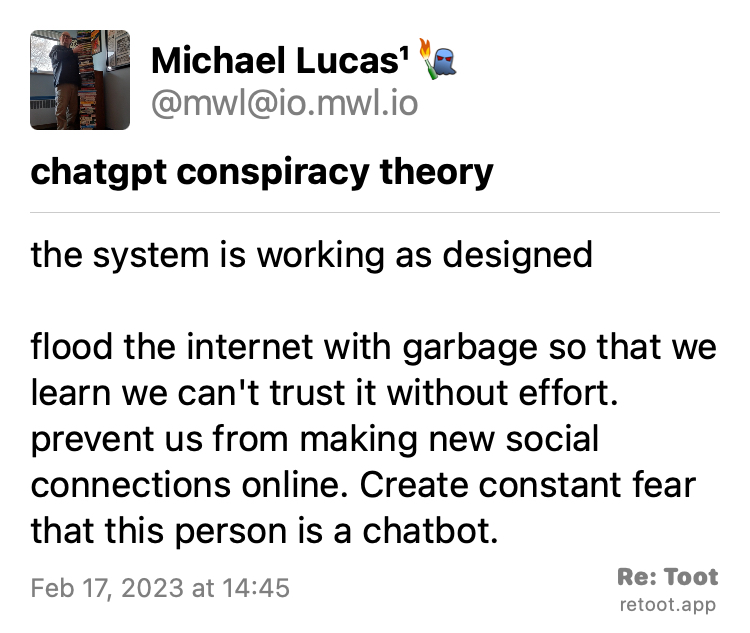
\includegraphics[keepaspectratio]{\%7B\%7Bsite.url\%7D\%7D/img/chat-conspiracy.jpg}}
\caption{Post by Michael Lucas¹. Content warning:
``EmojiString(stringValue: chatgpt conspiracy theory\{ \}, components:
{[}EmojiString.EmojiString.Component.text(chatgpt conspiracy theory\{
\}){]})''. ``the system is working as designed flood the internet with
garbage so that we learn we can't trust it without effort. prevent us
from making new social connections online. Create constant fear that
this person is a chatbot.'' Posted on Feb 17, 2023 at 14:45}
\end{figure}

I'm really getting doubtful of the efficacy of some approaches to this
sort of AI. We just saw \emph{Clarkesworld} have to slam its submissions
window shut indefinitely
\href{http://web.archive.org/web/20230222022224/https://arstechnica.com/information-technology/2023/02/sci-fi-becomes-real-as-renowned-magazine-closes-submissions-due-to-ai-writers/}{due
to a crapflood of ChatGPT-generated submissions}. At Johns Hopkins there
is an article posted
\href{http://web.archive.org/web/20230222055340/https://hub.jhu.edu/2023/02/20/chatgpt-in-higher-education-discussion/}{that
is optimistic about the use of ChatGPT in education} though it reads
like wishcasting to me. There are more stories about Microsoft's
instance of ChatGPT being welded to Bing that
\href{https://www.msn.com/en-gb/money/technology/microsoft-sets-new-limits-on-bing-chatgpt-to-prevent-unhinged-behavior/ar-AA17M0Nu}{is
acting unhinged}. All in all, this is becoming a rather fast moving
target.

Yeah, I am openly expressing doubts \emph{now}. With luck I will figure
out what I am doing. Time will tell, though\ldots{}
